\section{Approach}\label{sec:approach}

Credential ecosystem design involves three distinct concerns: what domain-level facts exist and how they relate, how those facts are grouped into credentials with defined subjects and claims, and which concrete credential format each credential uses. The metamodel separates these concerns into three layers: the \acf{DCL}, the \acf{CSL}, and the \acf{FSL}. The layered structure follows the multi-layer modeling principles introduced in \autoref{sec:multi-layer}: each layer is derived from the one above and carries its own intra-layer constraints. Constraints within and across layers are formalized as graph predicates that the Refinery framework (\autoref{sec:refinery}) can evaluate, yielding the three usage modes defined in \autoref{sec:functional-overview}. \autoref{fig:metamodel} shows the complete metamodel; the definitions below correspond to its elements layer by layer. Full Refinery encodings for all layer definitions, propagation rules, and constraint predicates are provided in the supplementary material.

\subsection{Domain Concept Layer}\label{sec:dcl}

Domain-level facts are modeled as a typed information graph at the first layer. The abstract metaclass \refi{Entity} has two concrete subclasses: \refi{Subject} and \refi{Value}. A \refi{Subject} is an entity that can anchor a credential, representing the person, organization, or thing about which claims are made. A \refi{Value} is an entity that serves as the target of a property. Each \refi{Entity} contains zero or more \refi{Prop} instances; each \refi{Prop} holds exactly one \refi{Value} through a containment reference and carries a trace link to the credential schema layer (\autoref{sec:csl}). The ternary predicate \refi{statement(s, p, v)} is satisfied when subject \(s\) owns property \(p\) and \(p\) contains value \(v\), with the well-formedness condition \(s \neq v\). The distinction between \refi{Subject} and \refi{Value} is inferred structurally: a propagation rule (\autoref{sec:refinery}) classifies any \refi{Entity} with no incoming value reference as a \refi{Subject}: a root of the property tree, and therefore a candidate credential subject at the \ac{CSL} layer.
A credential ecosystem must cover all domain-level facts; an entity unreachable from the rest of the graph represents a fact that no credential path connects to the subject, and therefore cannot be verified. The \refi{non_connected} error predicate (\autoref{sec:refinery}) enforces this: it flags any pair of entities not transitively reachable through the \refi{neighbours} relation, where two entities are neighbours if a \refi{statement} connects them in either direction. The \refi{no_self_loop} propagation rule prevents an entity from serving as both the owner and the value of the same property, a structurally meaningless configuration that would collapse the subject--value distinction. Together with the \(s \neq v\) condition in the \refi{statement} predicate, these constraints ensure that every \ac{DCL} instance is a connected, directed acyclic information graph with clear directionality from subjects to values. The \refi{cyclic} error predicate enforces acyclicity via transitive closure of the \refi{neighbours} relation. In terms of the usage modes (\autoref{sec:functional-overview}), \ac{DCL} constraints serve error identification: evaluating \refi{non_connected} on a partial specification with an orphaned entity returns \textbf{NOT\_OK}(\refi{non_connected(e1, e2)}), naming the unreachable pair and indicating where the domain model is incomplete.

In the housing subsidy scenario (\autoref{fig:teaser}, top), the \ac{DCL} instance models the Applicant as a \refi{Subject} with three properties: \refi{has_children} \(\to\) \refi{num_children} (family size), \refi{owns_property} \(\to\) \refi{property_area} (floor area), and \refi{earns} \(\to\) \refi{monthly_income} (employment income). Three statements capture the domain facts, one per property edge in the domain graph. Two domain constraints apply: \refi{property_area} \(\geq\) \refi{min_area(num_children)} links two properties across what will become separate credentials, and \refi{monthly_income} \(\geq\) \refi{threshold} establishes a privacy-sensitive eligibility check. All claim-layer structural constraints (connectivity, no self-loops) are satisfied.

\subsection{Credential Schema Layer}\label{sec:csl}

The \acf{CSL} models the partitioning of domain-level facts into credentials, each issued by a different authority and carrying a subset of the domain's claims. Each \ac{CSL} element is traced from a \ac{DCL} element: the abstract metaclass \refi{CredEntity} carries a mandatory \refi{trace} reference to exactly one \ac{DCL} \refi{Entity}, and each \ac{DCL} \refi{Prop} contains exactly one \refi{Claim} via \refi{Prop::trace}. This pair of cross-layer references ensures that every credential-layer element has a domain-level origin (\autoref{fig:metamodel}). \ac{CSL} mirrors the \ac{DCL} type structure: \refi{CredentialSubject} and \refi{CredentialValue} specialize \refi{CredEntity}, paralleling \ac{DCL}'s \refi{Subject} and \refi{Value}. A \refi{Claim} connects a source \refi{CredEntity} to a target \refi{CredentialValue}, mirroring the \ac{DCL} \refi{statement} predicate. Each \refi{CredentialSubject} optionally contains a \refi{Credential}, which itself holds exactly one \refi{Formatted_Credential} (\autoref{sec:fsl}).

Trace mappings do more than record provenance. Combined with Refinery's propagation rules, they actively derive \ac{CSL} structure from \ac{DCL} during model generation. Two propagation rules derive \ac{CSL} type assignments from \ac{DCL} structure. \refi{subject_traces_to_subject} infers \refi{CredentialSubject} when a \refi{CredEntity} traces to a \ac{DCL} \refi{Subject}; \refi{root_is_cred_subj} infers it when no \refi{Claim} targets the entity, mirroring the \ac{DCL} \refi{root_is_subj} at the credential level. The effect is that \ac{CSL} type assignments are derived from \ac{DCL} structure rather than independently specified: a credential entity's type is a consequence of its domain-layer origin.

Beyond type derivation, the metamodel enforces structural well-formedness through four predicates (two shadow, two error; \autoref{sec:refinery}). The shadow predicates mirror \ac{DCL} structure at the credential level: \refi{credential_statement} is true when a \refi{Claim} connects distinct source and target with the target typed as \refi{CredentialValue}; \refi{Root_cred_entity} holds when a \refi{CredEntity} is not targeted by any \refi{credential_statement}. The error predicates flag structural violations: \refi{no_empty_cred} flags a \refi{CredentialSubject} with no outgoing \refi{Claim}, and \refi{root_ent_doesnt_have_cred} flags a root entity without an associated \refi{Credential}; the anti-pattern catalog (\autoref{sec:anti-patterns}) classifies all five predicates by layer scope and kind. The error predicates catch structural violations that would otherwise propagate silently to downstream format assignment. When either fires, the framework reports the violation (e.g., \textbf{NOT\_OK}(\refi{no_empty_cred(cs)})) before format-specific constraints are even evaluated. In terms of the usage modes (\autoref{sec:functional-overview}), the shadow predicates (\refi{credential_statement}, \refi{Root_cred_entity}) derive structural facts in all three modes; the error predicates (\refi{no_empty_cred}, \refi{root_ent_doesnt_have_cred}) trigger in consistency checking and error identification.

In the housing subsidy scenario, three credentials partition the facts: FamilyStatusCred (civil registry: \refi{CS_Applicant}\(_1\), claim \refi{has_children}\(_1 \to\) \refi{num_children}\(_1\)), PropertyCred (land registry: \refi{CS_Applicant}\(_2\), claim \refi{owns_property}\(_1 \to\) \refi{property_area}\(_1\)), and IncomeCred (employer: \refi{CS_Applicant}\(_3\), claim \refi{earns}\(_1 \to\) \refi{monthly_income}\(_1\)). Each credential subject, claim, and value traces to its \ac{DCL} counterpart.

All three credential subjects trace to the same \ac{DCL} entity: \refi{trace(CS_Applicant_i, Applicant)} for \(i \in \{1,2,3\}\). Each claim traces to its corresponding property, and each credential value traces to its corresponding value. Entity alignment holds pairwise: \refi{aligned(CS_Applicant_i, CS_Applicant_j)} for all \(i \neq j\). The cross-property domain constraint (minimum floor area as a function of the number of children) now spans two credentials, requiring the verifier to combine claims from FamilyStatusCred and PropertyCred.

\subsection{Format-Specific Layer}\label{sec:fsl}

Each credential receives a concrete representation format at the third layer, the \acf{FSL}. The abstract metaclass \refi{Formatted_Credential} has five concrete subclasses (one per credential format in scope: AnonCreds, JSON-LD, JWT-VC, SD-JWT-VC, and mdoc), and each \refi{Credential} contains exactly one instance via the \refi{format[1]} containment. These formats differ along a design-relevant axis: \emph{selective disclosure} (revealing a subset of claims) versus \emph{predicate proofs} (proving a comparison such as \refi{monthly_income} \(\geq\) \refi{threshold} without disclosing the value). Format capabilities follow from the analysis in \autoref{sec:vcdm}: only AnonCreds supports predicate proofs natively; the remaining formats provide selective disclosure only. Formats lacking predicate proofs force issuers to pre-compute boolean claims, restructuring the domain concept layer (\autoref{sec:cross-layer}). Unlike the \ac{DCL} and \ac{CSL}, the format-specific layer does not yet carry intra-layer structural constraints; its role in the metamodel is different. \ac{FSL} elements participate in cross-layer predicates (\autoref{sec:cross-layer}), carry governance annotations as typed containment, and their capability predicates feed the propagation rules that narrow the format design space during generation. The layer is a metamodel component with cross-layer predicate participation and governance semantics, not a lookup table mapping credentials to format labels.

The metamodel encodes format capabilities as six derived predicates over the class hierarchy, each capturing a functional property that at least one governance framework or domain requirement in the running example imposes:

\begin{table}[htb]
\caption{\ac{FSL} capability predicates derived from the format class hierarchy.}
\small
\setlength{\tabcolsep}{4pt}
\begin{tabularx}{\columnwidth}{LL}
\toprule
Predicate & Capability \\
\midrule
{supports\_predicate\_proof} & Predicate proof (e.g., {monthly\_income} \(\geq\) {threshold} without
disclosure) \\
{supports\_selective\_disclosure} & Selective disclosure of claim subsets \\
{conforms\_vcdm} & W3C VCDM 2.0 data model conformance \\
{supports\_zkp} & Zero-knowledge proof support \\
{supports\_offline\_verification} & Offline verification without network access \\
{supports\_multi\_credential\_proof} & Cross-credential predicate evaluation \\
\bottomrule
\end{tabularx}
\end{table}

Propagation rules narrow the format design space during generation: requiring predicate proof support on IncomeCred eliminates all formats except AnonCreds, which does not conform to W3C \ac{VCDM} 2.0, setting up the governance conflict in \autoref{sec:headlines}. Three governance annotation classes (\refi{EidasMandate}, \refi{PrivacyRequirement}, \refi{VcdmConformance}) attach regulatory requirements to individual credentials as typed markers for error identification and \ac{DSE}.

In the housing subsidy scenario, format assignments are governance-driven. FamilyStatusCred and PropertyCred are assigned SD-JWT-VC under the eIDAS \ac{ARF} mandate; both formats mandated by the \ac{ARF} (SD-JWT-VC and mdoc) lack predicate proof support; we use SD-JWT-VC as representative \citep{noauthor_eu-digital-identity-walleteudi-doc-architecture-and-reference-framework_2026}. IncomeCred is the conflict site analyzed in \autoref{sec:headlines}: the income threshold check requires predicate proof capability that the ARF-mandated format does not provide.

\subsection{Cross-Layer Constraints as Graph Predicates}\label{sec:cross-layer}

\begin{figure}
\centering
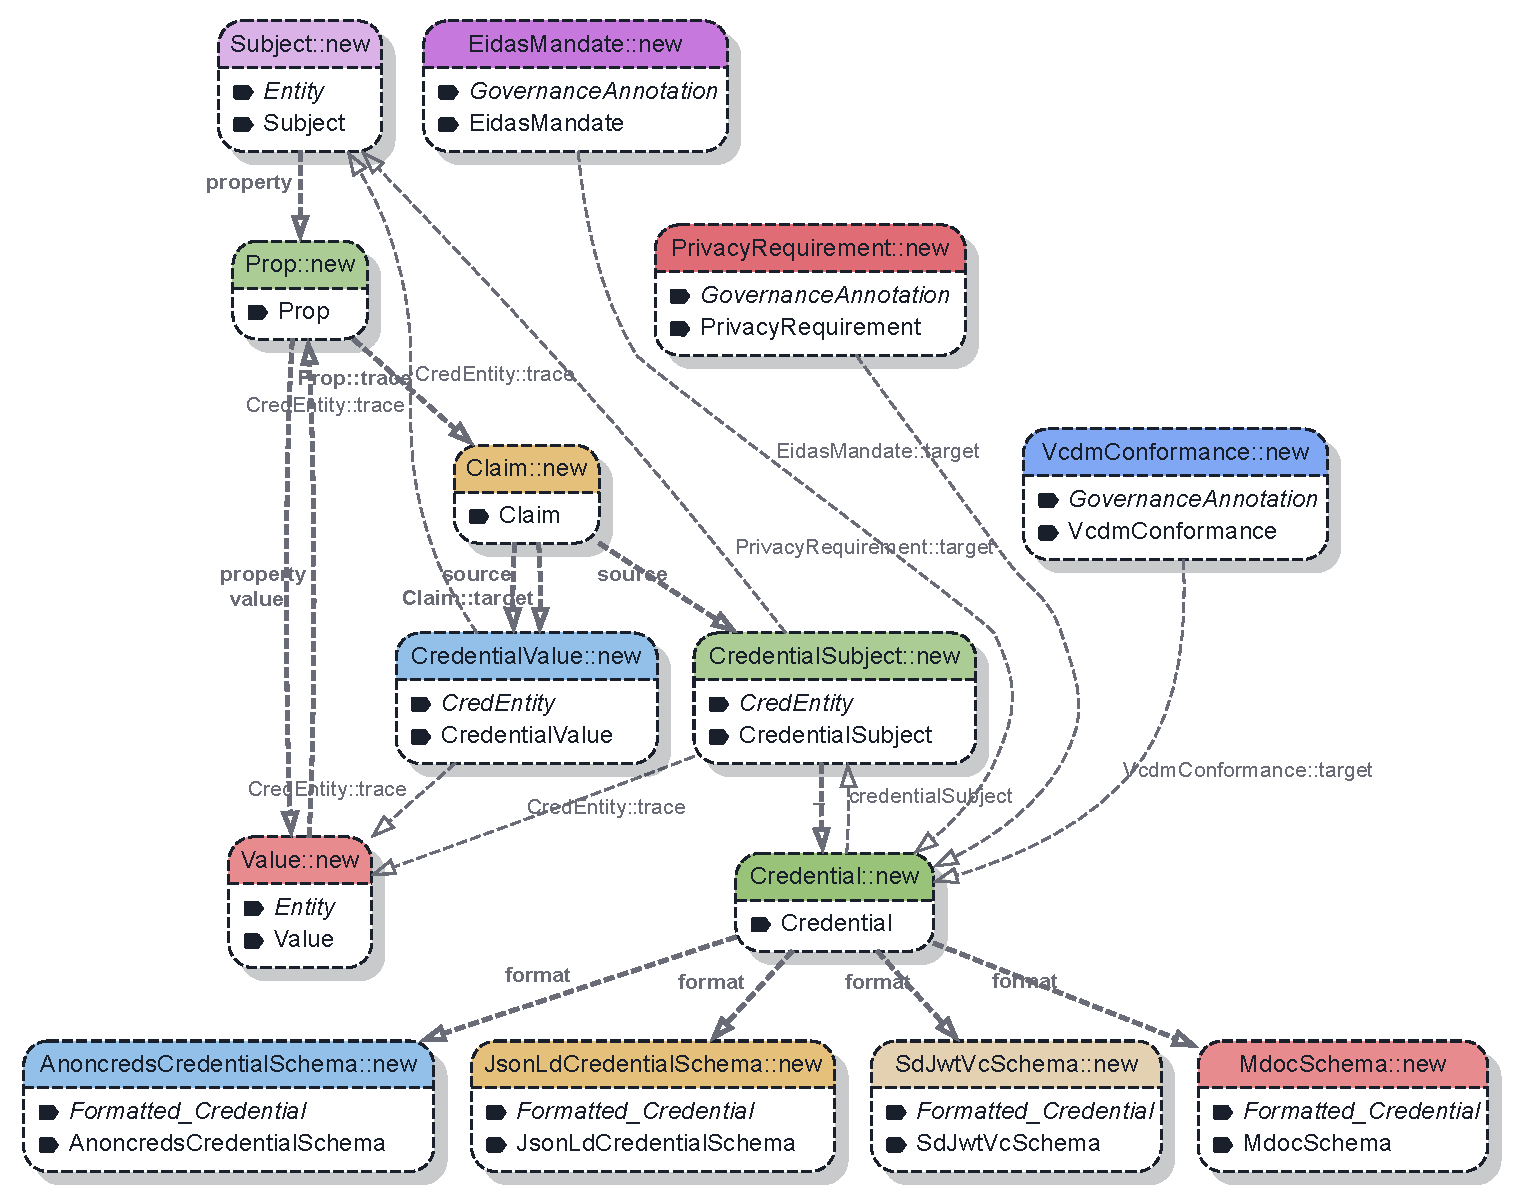
\includegraphics[width=1\linewidth,height=\textheight,keepaspectratio,alt={The three-layer type graph. The  models facts as a typed information graph; the  partitions facts into credentials with subject bindings and trace mappings; the  assigns concrete formats with capability predicates and governance annotations.}]{pandoc/assets/fig_metamodel.pdf}
\caption{The three-layer type graph. The \ac{DCL} models facts as a typed information graph; the \ac{CSL} partitions facts into credentials with subject bindings and trace mappings; the \ac{FSL} assigns concrete formats with capability predicates and governance annotations.}\label{fig:metamodel}
\end{figure}

Cross-layer constraints are predicates whose variables reference elements from more than one metamodel layer; they capture design requirements that no single-layer check can express. The following table classifies the constraints exercised in the housing subsidy scenario by source and scope:

\begin{table}[htb]
\caption{Cross-layer constraint taxonomy. C1--C3 are metamodel-enforced; C4 is
grounded in regulation; C5--C7 originate from independent governance
frameworks; C8 and C9 are cross-layer results.
\label{tab:constraint_taxonomy}}
\small
\setlength{\tabcolsep}{4pt}
\begin{tabularx}{\columnwidth}{LLLL}
\toprule
\# & Constraint & Source & Layers \\
\midrule
C1 & Entity alignment & Structural & DCL\(\leftrightarrow\)CSL \\
C2 & Trace consistency & Structural & DCL\(\rightarrow\)CSL \\
C3 & No empty credential & Structural & CSL \\
C4 & Cross-credential value dep. & Domain rule & DCL horiz. \\
C5 & Format mandate & eIDAS \ac{ARF} & FSL \\
C6 & Predicate proof required & \ac{GDPR} Art. 5(1)(c) & DCL\(\leftrightarrow\)FSL \\
C7 & VCDM conformance & W3C VCDM 2.0 & CSL\(\leftrightarrow\)FSL \\
C8 & \textbf{Governance conflict} & eIDAS+GDPR+W3C & FSL \\
C9 & Cross-credential predicate gap & Format limitation & DCL\(\leftrightarrow\)FSL \\
\bottomrule
\end{tabularx}
\end{table}

Constraints C1--C3 are structural (metamodel-enforced). C4 is a domain rule grounded in government regulation. C5--C7 each originate from a different governance framework. C8 and C9 are cross-layer results: they emerge only when constraints from multiple sources and layers are checked jointly. \autoref{sec:headlines} develops C8 and C9 as the paper's headline results.

\autoref{fig:teaser} traces all three usage modes on the constraint table above. Consistency checking on the partial specification returns \textbf{OK}. Fixing IncomeCred to SD-JWT-VC triggers error identification: the framework returns \textbf{NOT\_OK}(\refi{governance_conflict(IncomeCred, income_format)}), naming the conflict site where C5, C6, and C7 cannot be simultaneously satisfied. Leaving IncomeCred's format open and running \ac{DSE} with \refi{C5} \(\wedge\) \refi{C6} \(\wedge\) \refi{C7} returns \textbf{UNVIABLE}. Relaxing C6, the framework generates configurations assigning SD-JWT-VC to all three credentials.

The predicates defined in the preceding sections (\refi{non_connected}, \refi{no_empty_cred}, \refi{root_ent_doesnt_have_cred}) operate within a single layer using the Refinery mechanisms introduced in \autoref{sec:refinery}. The cross-layer predicates below combine elements from multiple layers and fall into three categories defined in \autoref{sec:refinery}: \emph{propagation rules}, \emph{shadow predicates}, and \emph{error predicates}. This classification determines which usage mode (\autoref{sec:functional-overview}) each predicate serves.

A \refi{Claim} that connects to a \refi{CredEntity} tracing to the wrong \ac{DCL} \refi{Entity} is a silent design error: each layer is well-formed individually, but the cross-layer mapping is broken. Two propagation rules prevent this by negative elimination. The target consistency rule enforces that if \refi{trace(p, c)} and \refi{value(p, e)} hold (where \refi{trace(p, c)} denotes \refi{Prop::trace} and \refi{trace(t, e)} below denotes \refi{CredEntity::trace}), then any \refi{CredEntity} \(t\) for which \(\neg\)\refi{trace(t, e)} holds is excluded as \(c\)'s target; the source rule is dual over \refi{property(e, p)}. In the running example, the \refi{Claim} tracing to \refi{has_children} can only target a \refi{CredEntity} tracing to \refi{num_children}, not one tracing to \refi{property_area}. Both rules operate by negative elimination (\autoref{sec:refinery}): bindings inconsistent with committed traces are excluded before generation explores them.

The shadow predicate \refi{aligned} formalizes cross-authority subject identity: \refi{aligned(ce1, ce2)} holds when two distinct \refi{CredEntity} instances satisfy \refi{trace(ce1, e)} \(\wedge\) \refi{trace(ce2, e)} for some \ac{DCL} \refi{Entity} \(e\). In the running example, \refi{aligned(CS_Applicant_i, CS_Applicant_j)} holds for all \(i \neq j\). A second shadow predicate, \refi{common_parent}, holds when two \refi{Prop} instances' traced \refi{Claim} instances share a source \refi{CredEntity}, capturing co-location within a single credential. Both feed the anti-pattern analysis (\autoref{sec:evaluation}); \refi{aligned} additionally feeds \refi{cross_cred_predicate_gap} below.

Some design problems are invisible at any single layer. When a domain constraint spans two credentials (\refi{property_area} \(\geq\) \refi{f(num_children)} requires combining claims from FamilyStatusCred and PropertyCred), the design depends on a format capability that may not exist. The shadow predicate \refi{cross_cred_predicate_gap} detects this: \refi{cross_cred_predicate_gap(c1, c2)} fires when \refi{aligned(cs1, cs2)} and at least one credential's format lacks multi-credential proof support. No deployed format supports cross-credential arithmetic (AnonCreds supports multi-credential \emph{presentation} but not cross-credential \emph{computation}), so the predicate fires for every aligned pair, making a structural limitation of the current format space visible. As a shadow predicate, it records a condition whose severity depends on domain requirements; \autoref{sec:headlines} develops this as the second headline result.

Format capability propagation rules apply the same negative elimination mechanism (\autoref{sec:refinery}) at the format level. When a governance annotation demands a capability, incompatible format classes are eliminated: requiring \refi{supports_predicate_proof} on IncomeCred excludes SD-JWT-VC, JWT-VC, mdoc, and JSON-LD, leaving only AnonCreds. When no format in scope satisfies a required capability, the only workaround is restructuring the domain concept layer, replacing a numeric property with pre-computed boolean claims, a cross-layer design consequence that \autoref{sec:headlines} develops as the first headline result.
